\chapter{Implementação}\label{cap:implementacao}


Este capítulo descreve a implementação usada para produzir e analisar os dados. O sistema reúne dois fluxos: o legado, baseado em atributos de movimento e fluxo óptico, e o espacial, que transforma profundidade em um mapa de ocupação e em caminhos para o PX4. Os dois compartilham o mesmo ambiente simulado, mas respondem a perguntas diferentes.

\section{Ambiente experimental}

O PX4 atua como piloto automático \cite{Meier8092}. O Gazebo simula o ambiente e os sensores \cite{Koenig7803}, e o ROS~2 fornece a camada de comunicação \cite{Macenski2022}.


Os experimentos usam SITL, com PX4 como piloto automático, Gazebo como ambiente físico e ROS~2 como camada de comunicação. O computador do laboratório possui processador Intel Core i7-14700K, com 20 núcleos e 28 \textit{threads}, 64~GB de memória de acesso aleatório (RAM) e uma unidade de processamento gráfico (GPU) NVIDIA GeForce RTX 4080 SUPER com 16~GB de memória de vídeo.

O ambiente simulado utilizado nos experimentos foi desenvolvido com o apoio do professor Eduardo Charles Vasconcellos (UFRJ), especialmente na configuração do cenário, do UAV e dos componentes relacionados ao voo autônomo.

O sistema executa Ubuntu 22.04.5 com suporte de longo prazo (LTS) no \textit{Windows Subsystem for Linux}~2 (WSL~2), com kernel 6.6.87.2. Foram usados o PX4 no commit \texttt{e2708705a8ca625854f1129fd9dde2ae8ae16d59}, ROS~2 Humble, Gazebo Harmonic 8.10.0 e Python 3.10.12. O veículo é o \texttt{x500\_mono\_cam} e o cenário é o \texttt{baylands}.

\section{Pipeline de voo e coleta}

O controlador recebe posição local e dados inerciais do PX4, publica comandos no modo \textit{Offboard} e processa imagens de uma câmera RGB monocular frontal. No fluxo legado, a imagem fornece o fluxo óptico usado pela lógica reativa. No fluxo espacial, ela alimenta o estimador monocular, e o A* substitui a decisão reativa de desvio. Uma câmera de profundidade alinhada fornece os alvos tabulares e a referência da avaliação monocular. Na bateria espacial de referência, essa profundidade também alimenta mapa e A* para validar a geometria e o planejamento. Ela não entra na MLP nem no estimador monocular.

O planejador recebe uma sequência configurável de objetivos. Na bateria espacial de referência, foram usados três objetivos relativos no sistema norte-leste-baixo (NED), em metros: $(-25,25,-1{,}5)$, $(-50,70,-1{,}5)$ e $(-25,25,-1{,}5)$. O A* fornece pontos de posição ao modo \textit{Offboard}, enquanto o PX4 mantém a estabilização do veículo. A configuração da bateria de referência usa raio horizontal de segurança de 1,25~m, banda e inflação verticais de 0,10~m no mapa de planejamento e tolerância vertical de 0,50~m. Essas margens foram escolhidas antes da bateria final: valores verticais maiores faziam as copas das árvores bloquear o plano de voo mesmo quando havia separação em altura.

A base tabular consolidada contém 40 execuções completas e 1.234 intervalos sincronizados. Trinta e cinco execuções compõem o treino no marco final, duas formam a validação fixa e três formam o teste fixo. O rótulo de 40 execuções representa o total disponível nesse marco. Separadamente, o diretório espacial contém 103 diretórios de execuções completas, produzidos em diferentes etapas de desenvolvimento, treinamento, diagnóstico e validação. Ele funciona como arquivo experimental e não como um segundo conjunto homogêneo de repetições ou como 103 repetições equivalentes.

Os quatro exemplos preservam os registros históricos identificados nas próprias figuras: 15/07/2026 às 16:34:28, 21/07/2026 às 12:18:51 e 23/07/2026 às 12:55:06 e 23:54:09. São logs de voo do fluxo legado, distintos das linhas sincronizadas da base tabular de 40 execuções. A seleção preserva os exemplos da versão comentada, sem se basear no erro dos modelos.

A trajetória é reconstruída pela soma dos deltas de posição, com origem relativa em zero. A vista superior explicita ida e retorno: o aspecto de X corresponde a cruzamentos na projeção dos percursos, não a uma trajetória que termina nesses cruzamentos. Os quatro pontos finais ficam a menos de 2 m da origem horizontal. Não se inferem colisões nem coincidência temporal a partir de cruzamentos bidimensionais.

A auditoria encontrou 6, 4, 5 e 1 intervalos de tempo não finitos, não positivos ou superiores a 1 s, respectivamente. Por isso, a linha é interrompida nesses limites, sem substituir ou eliminar os deltas usados na soma espacial. Os maiores deslocamentos registrados por atualização ficam entre 0,57 e 0,61 m. Isso não permite recuperar o tempo físico perdido nem garantir a ausência de outras falhas de aquisição. Esses logs são usados aqui para ilustração e não alteram os resultados tabulares ou espaciais consolidados.

\begin{figure}[htb]
    \centering
    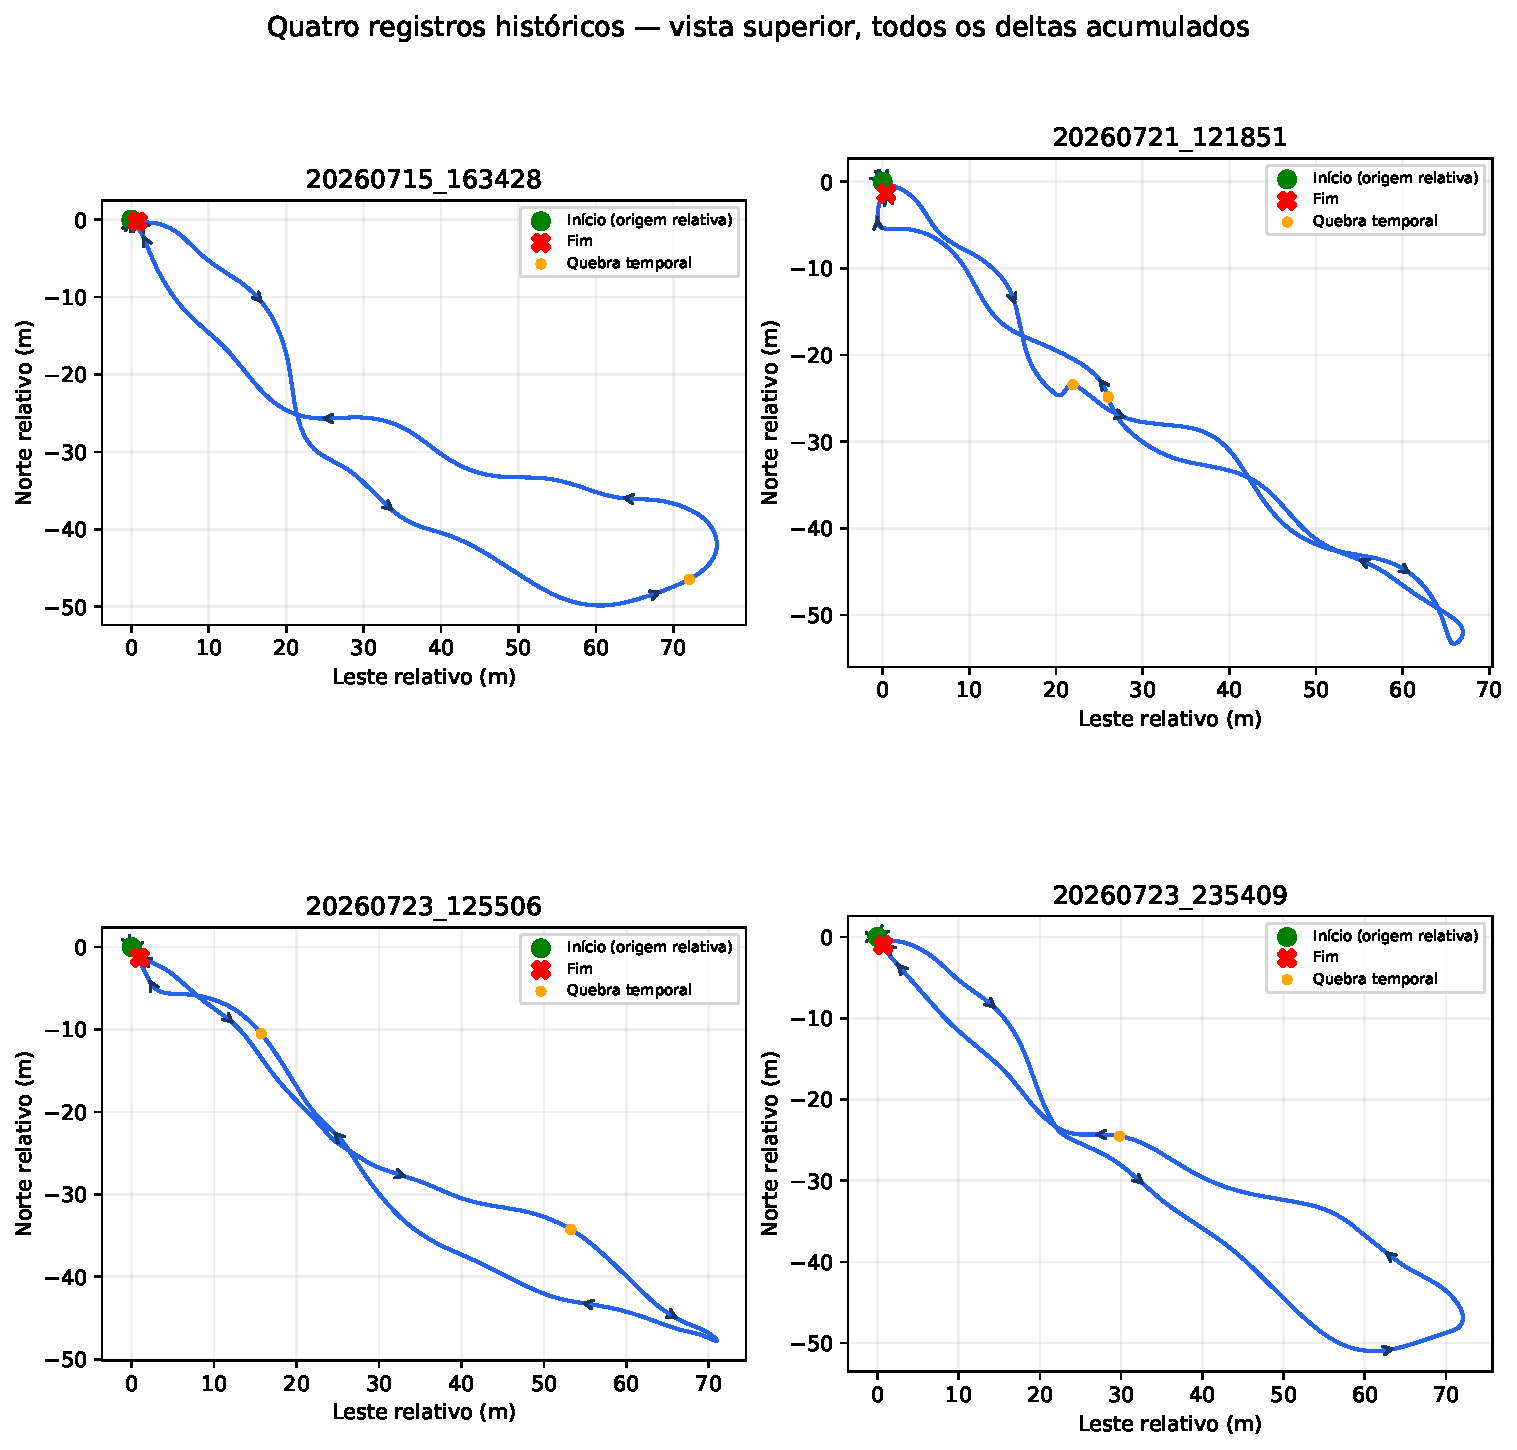
\includegraphics[width=\textwidth]{figuras/metodologia_trajetorias.pdf}
    \caption{Trajetórias históricas em vista superior, com início, fim, sentido e quebras temporais identificados. As coordenadas são deslocamentos acumulados relativos.}
    \label{fig:metodologia-trajetorias}
    \legend{Fonte: elaborado pelo autor.}
\end{figure}

A Figura~\ref{fig:metodologia-imu} mostra diferenças de velocidade angular, em rad/s, nas mesmas execuções. Não se trata de velocidades absolutas nem de integrais do giroscópio. Amostras nos limites temporais inválidos não são ligadas pela curva.

\begin{figure}[htb]
    \centering
    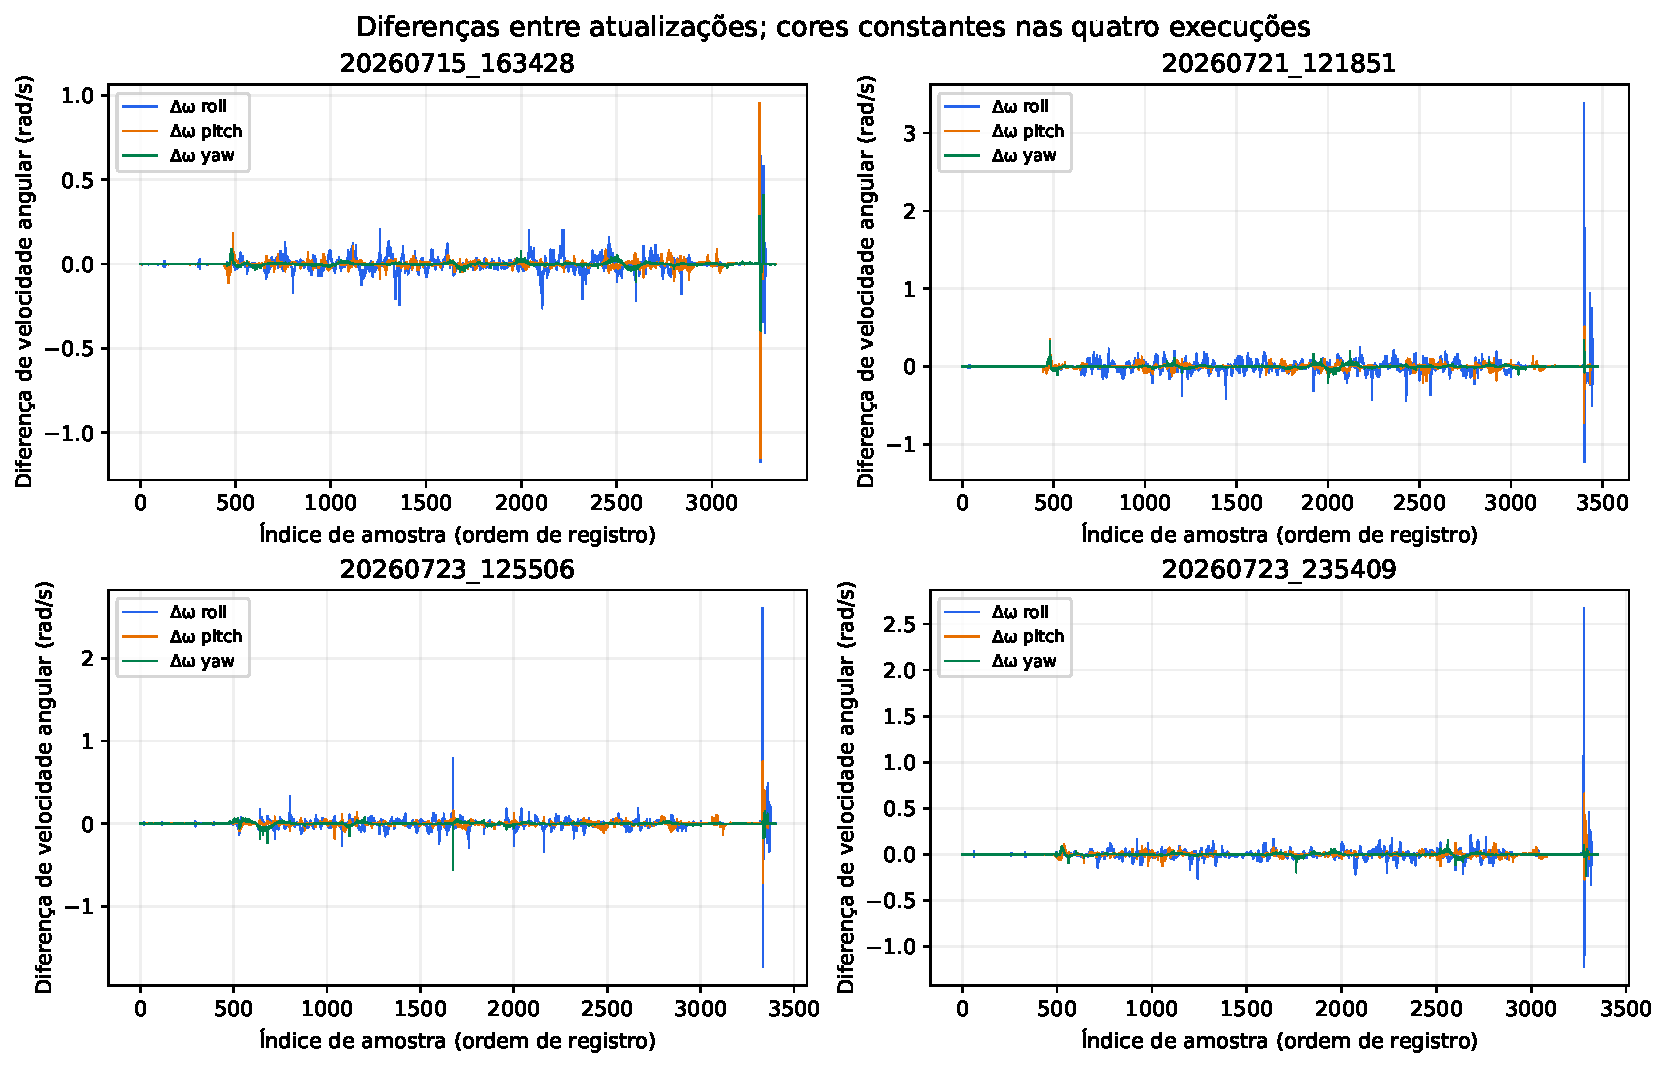
\includegraphics[width=\textwidth]{figuras/metodologia_imu.pdf}
    \caption{Diferenças das velocidades angulares de roll, pitch e yaw nas mesmas quatro execuções. As cores são constantes. O eixo horizontal usa a ordem das amostras, e não um tempo reconstruído a partir dos intervalos inválidos.}
    \label{fig:metodologia-imu}
    \legend{Fonte: elaborado pelo autor.}
\end{figure}


\begin{figure}[htbp]
\centering
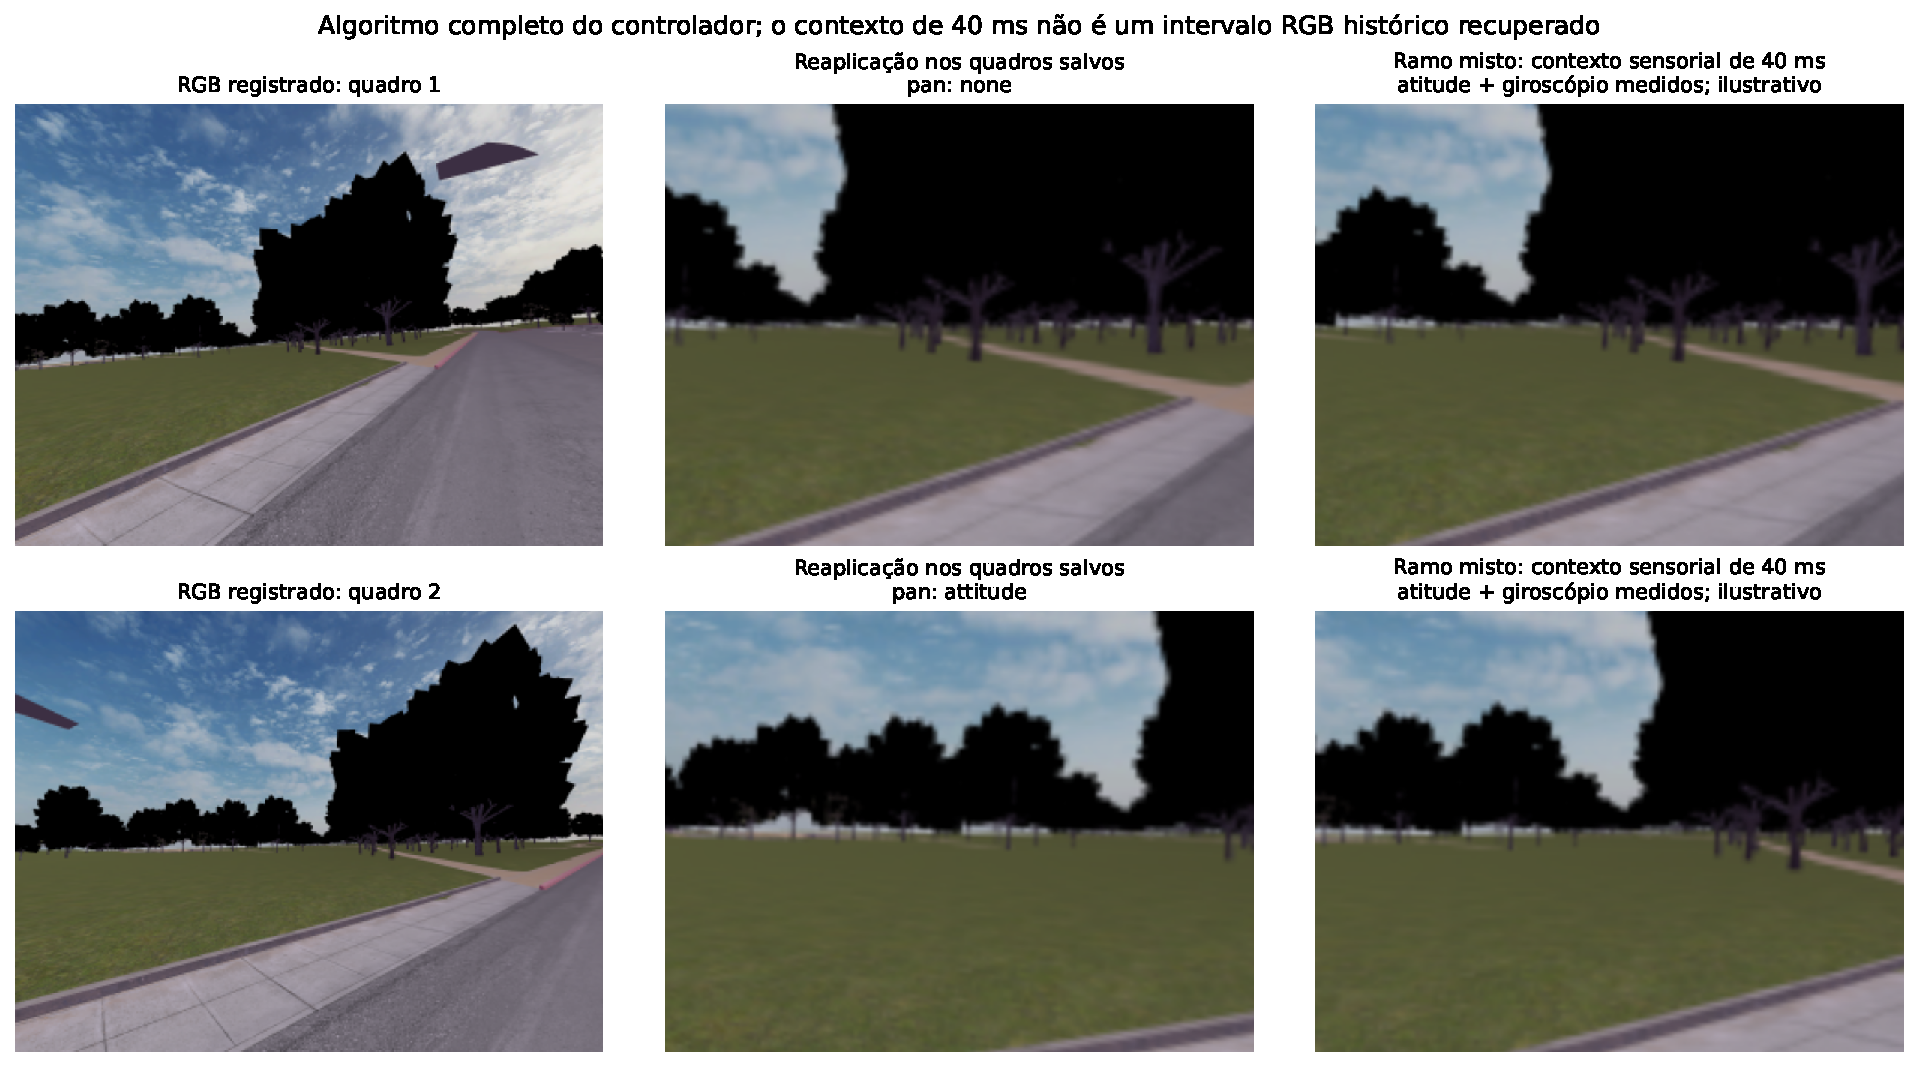
\includegraphics[width=.95\linewidth]{figuras/metodologia_compensacao_rotacao.pdf}
\caption{Algoritmo completo de compensação em dois quadros RGB registrados, usando atitude e giroscópio medidos no ULog correspondente. A coluna central respeita o intervalo de 0,66 s entre os quadros salvos, para o qual a regra original usa apenas a diferença de yaw. A coluna direita exercita a mistura atitude--giroscópio com contexto sensorial medido de 40 ms, explicitamente ilustrativo.}
\label{fig:compensacao-revisada}
\end{figure}
A Figura~\ref{fig:compensacao-revisada} reaplica os corpos originais das funções do controlador para normalização do yaw, seleção/mistura de fontes e construção da homografia. O ULog fornece atitude e giroscópio medidos. Os quadros armazenados estão separados por 0,66 s, acima do limite original de 0,25 s para mistura com giroscópio. A reaplicação respeita esse limite. Uma coluna separada demonstra a mistura completa com medições tomadas em uma janela de 40 ms, que não representa um instante RGB anterior recuperado. O RGB registrado em 320 por 240 pixels é ampliado para a geometria de entrada da demonstração, sem recuperar detalhe perdido. A ordem exata dos callbacks ROS e as imagens intermediárias não foram preservadas, portanto não se afirma identidade com a saída histórica online. O estimador denso continua recebendo o RGB original.

\begin{figure}[htbp]
\centering
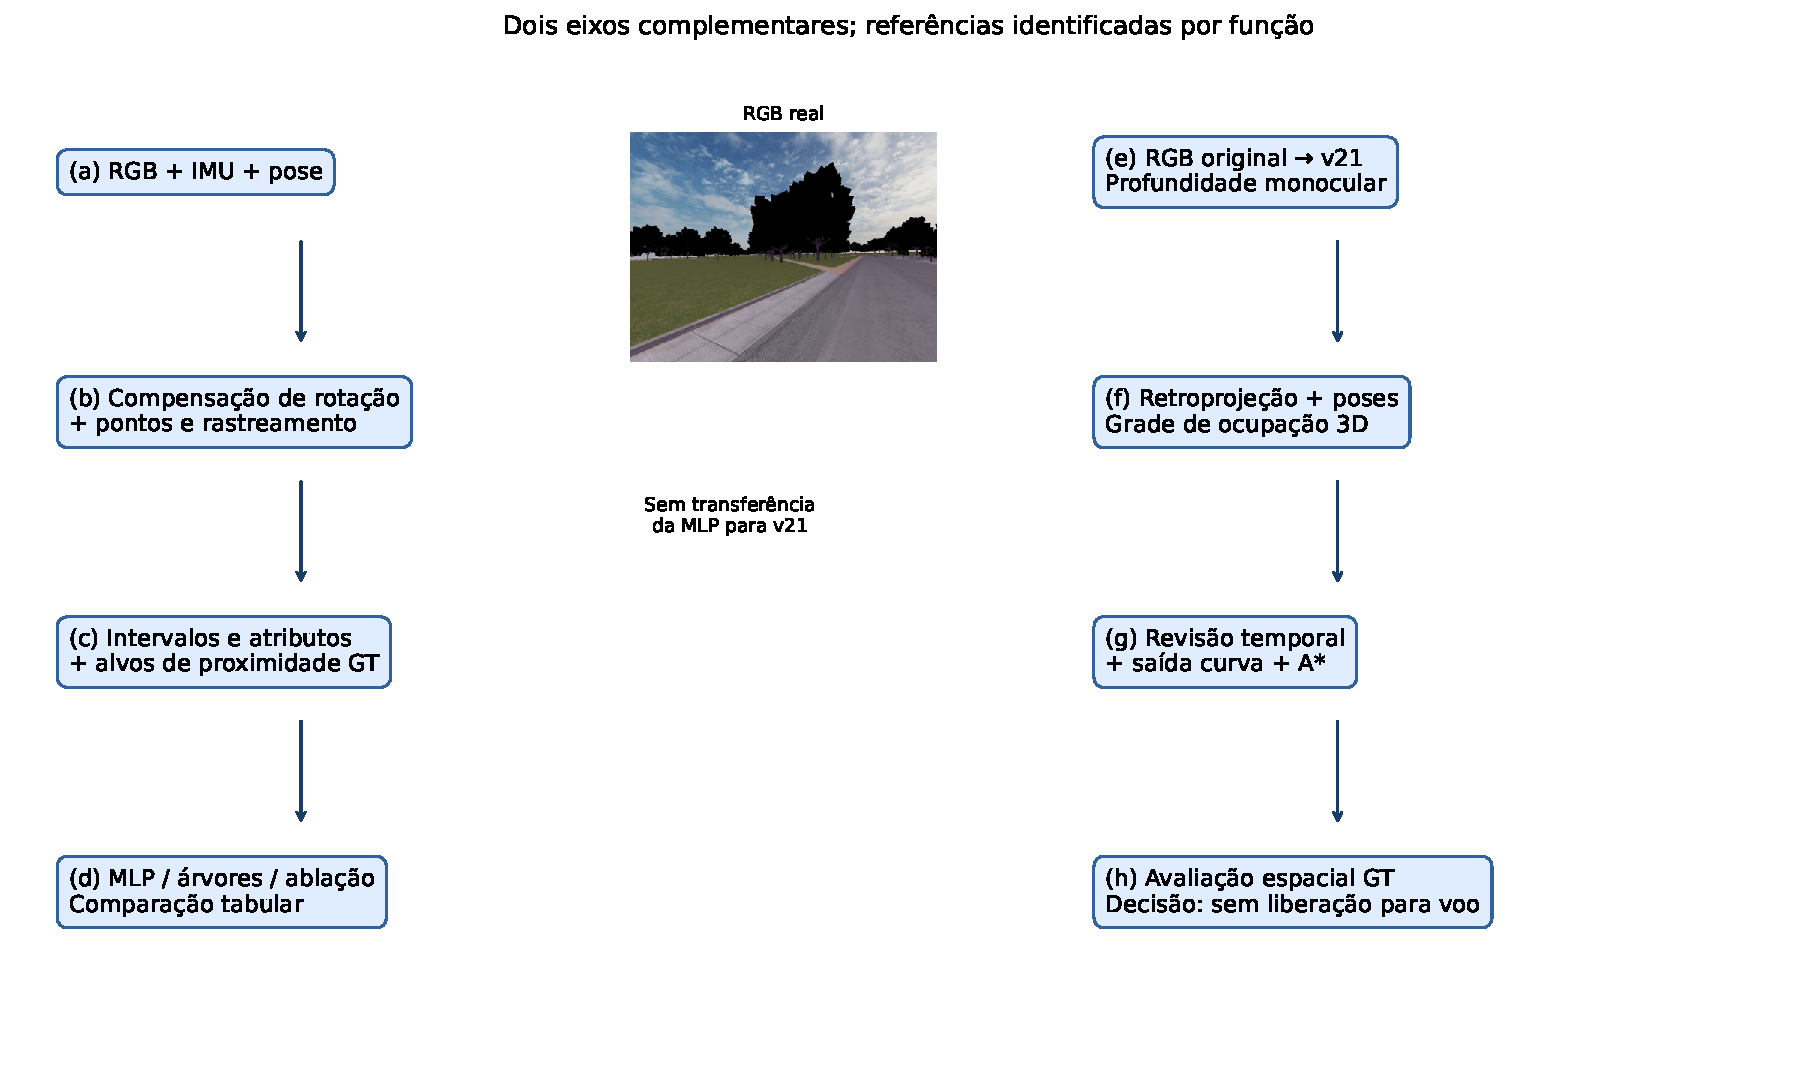
\includegraphics[width=.95\linewidth]{figuras/metodologia_fluxograma_completo.pdf}
\caption{Fluxo dos dois eixos, com etapas identificadas e quadro RGB real como exemplo. O GT fornece alvos tabulares e referência de avaliação espacial, sem escolher os caminhos monoculares.}
\label{fig:fluxograma-revisado}
\end{figure}
Na Figura~\ref{fig:fluxograma-revisado}, (a)--(d) organizam sinais, compensação, intervalos e comparação tabular. Os grupos incluem sincronização, movimento, IMU/atitude, fluxo/risco, diferença de imagem e comandos. No ramo (e)--(h), o RGB alimenta a rede densa, a pose permite a retroprojeção e o mapa recebe revisão temporal antes do planejamento. A MLP tabular não alimenta a rede v21.

\section{Processamento visual}

As imagens passam por estabilização com uma homografia calculada a partir da orientação do veículo. A saída possui resolução de $640\times480$ pixels e fator de aproximação de 1,25. A compensação reduz o fluxo causado pela rotação do drone e facilita a análise do movimento ligado à translação e à cena.

Os pontos de interesse são posições da imagem com variação de intensidade em duas direções, como cantos, e não objetos semanticamente reconhecidos. Eles são detectados por Shi--Tomasi \cite{ShiTomasi1994}, com até 180 pontos, qualidade mínima de 0,01, distância mínima de 12 pixels e bloco de 8 pixels. O rastreamento usa Lucas--Kanade piramidal \cite{LucasKanade1981}, janela de $21\times21$ pixels, três níveis adicionais de pirâmide e término após 20 iterações ou erro inferior a 0,04. O sistema registra quantidade e retenção de pontos, estatísticas do módulo do fluxo, componente radial e indicador heurístico de aproximação associado a cada ponto. Esse indicador combina expansão radial, posição na imagem e movimento do veículo no fluxo reativo legado. Não é uma probabilidade calibrada de colisão e não representa o planejador espacial.

Uma versão reduzida da diferença entre imagens estabilizadas também é armazenada. A partir dela são calculados média, desvio padrão, média do valor absoluto e percentil 90 do valor absoluto. A rede recebe esses descritores, e não os pixels completos.

\section{Sincronização e armazenamento}

O coletor associa cada intervalo RGB ao mapa de profundidade mais recente. Amostras sem fluxo, sem profundidade, com profundidade reutilizada ou tempos inválidos são descartadas. Os intervalos RGB e de profundidade precisam ser positivos e menores ou iguais a 0,5~s. A diferença temporal entre profundidade e RGB não pode ultrapassar 0,08~s.

Os dados são gravados em arquivos NumPy com mapeamento em memória. Cada execução possui um manifesto \textit{JavaScript Object Notation} (JSON) com esquema, quantidade de amostras, parâmetros e nomes dos vetores. Esse formato permite ler as execuções sem manter todas as imagens e matrizes na RAM e também permite ignorar uma execução incompleta.

A Figura~\ref{fig:metodologia-intervalos} apresenta a duração dos intervalos nas execuções completas.

\begin{figure}[htb]
    \centering
    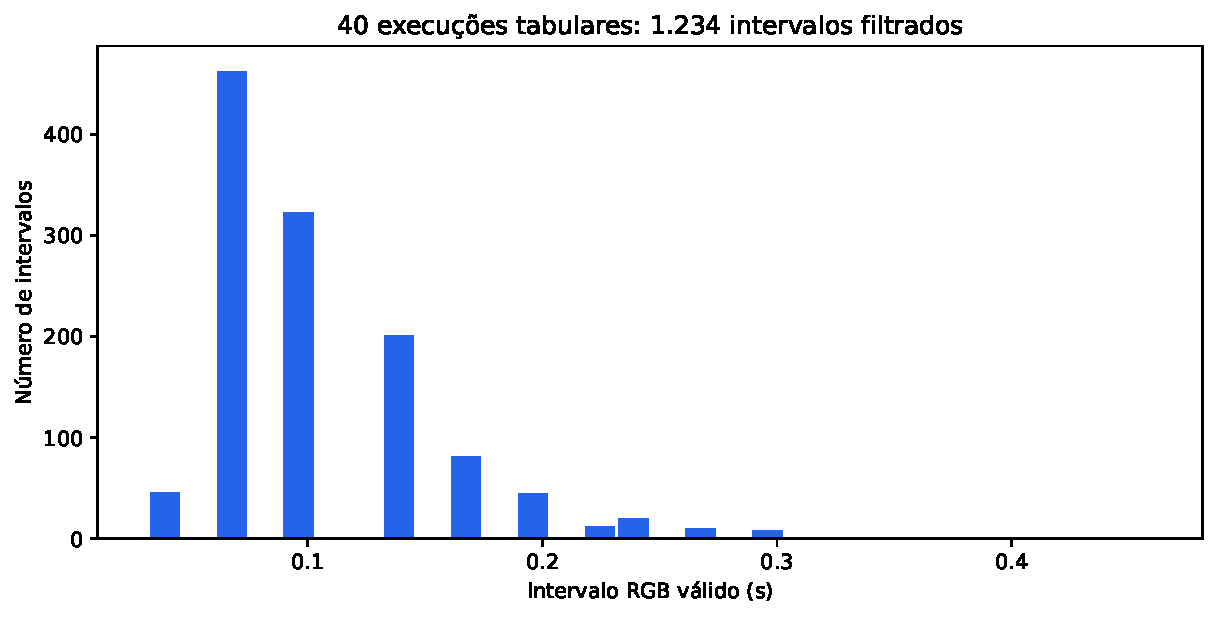
\includegraphics[width=\textwidth]{figuras/metodologia_intervalos_visuais.pdf}
    \caption{Distribuição dos 1.234 intervalos RGB válidos da base tabular histórica de 40 execuções, após os filtros documentados.}
    \label{fig:metodologia-intervalos}
    \legend{Fonte: elaborado pelo autor.}
\end{figure}

A Figura~\ref{fig:metodologia-sincronizacao} coloca na mesma sequência o percentil 90 do fluxo visual e a variação de pixels com profundidade inferior a 5~m. O gráfico serve para inspecionar o pareamento produzido, sem pressupor uma relação causal entre as duas grandezas.

\begin{figure}[htb]
    \centering
    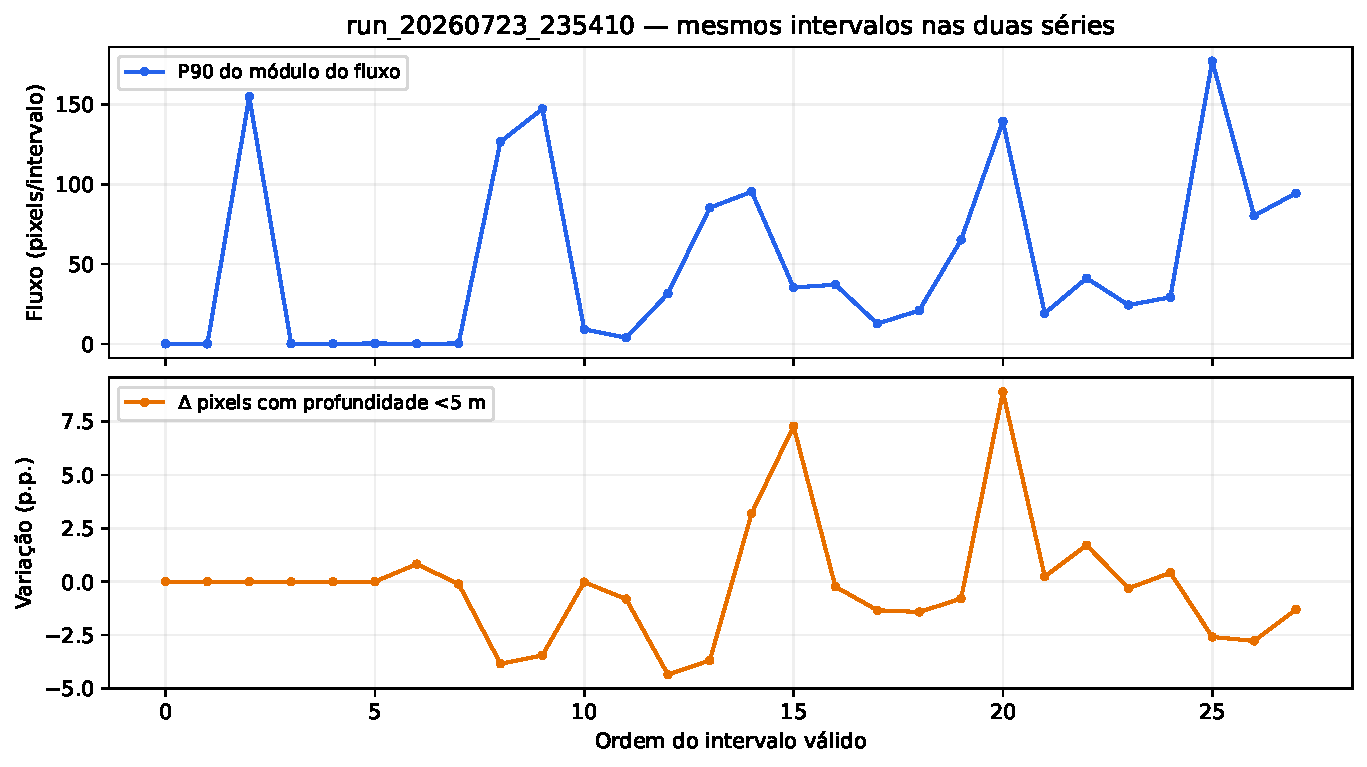
\includegraphics[width=\textwidth]{figuras/metodologia_sincronizacao.pdf}
    \caption{P90 do módulo do fluxo e variação da proporção de pixels a menos de 5 m nos mesmos intervalos válidos da última execução cronológica com pelo menos dez intervalos. Os eixos verticais têm unidades diferentes.}
    \label{fig:metodologia-sincronizacao}
    \legend{Fonte: elaborado pelo autor.}
\end{figure}


\begin{figure}[htbp]
\centering
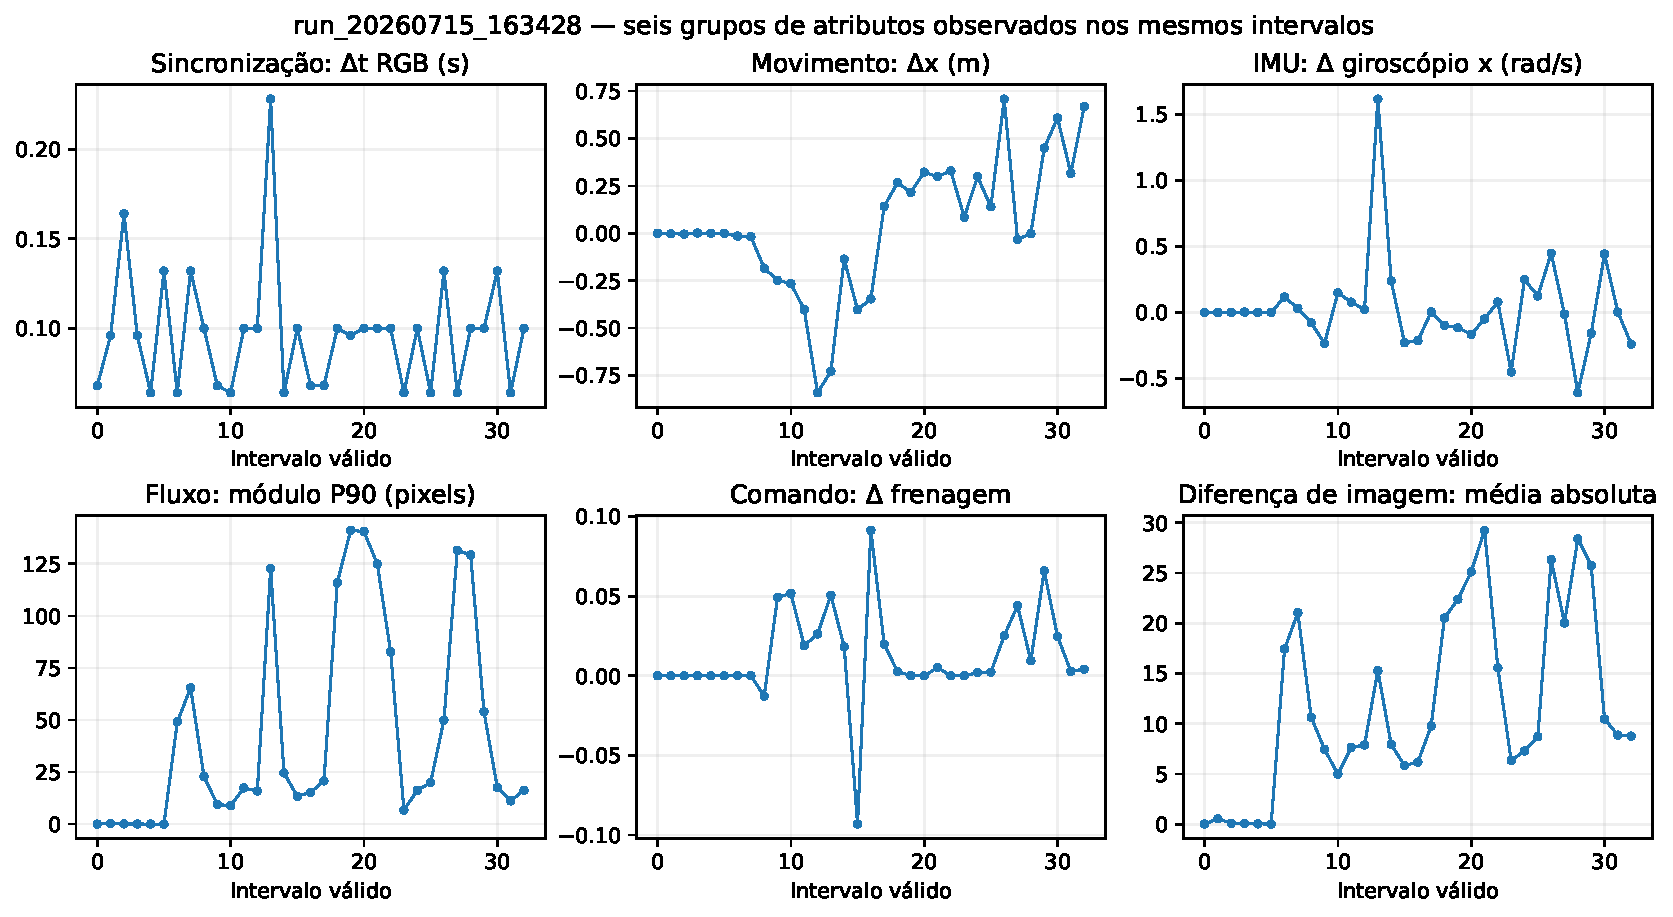
\includegraphics[width=.95\linewidth]{figuras/metodologia_grupos_sinais.pdf}
\caption{Exemplos reais dos seis grupos de entradas no registro de 15/07/2026 às 16:34:28. Os gráficos compartilham a ordem dos intervalos válidos, sem implicar causalidade entre séries.}
\label{fig:grupos-revisados}
\end{figure}

\begin{figure}[htbp]
\centering
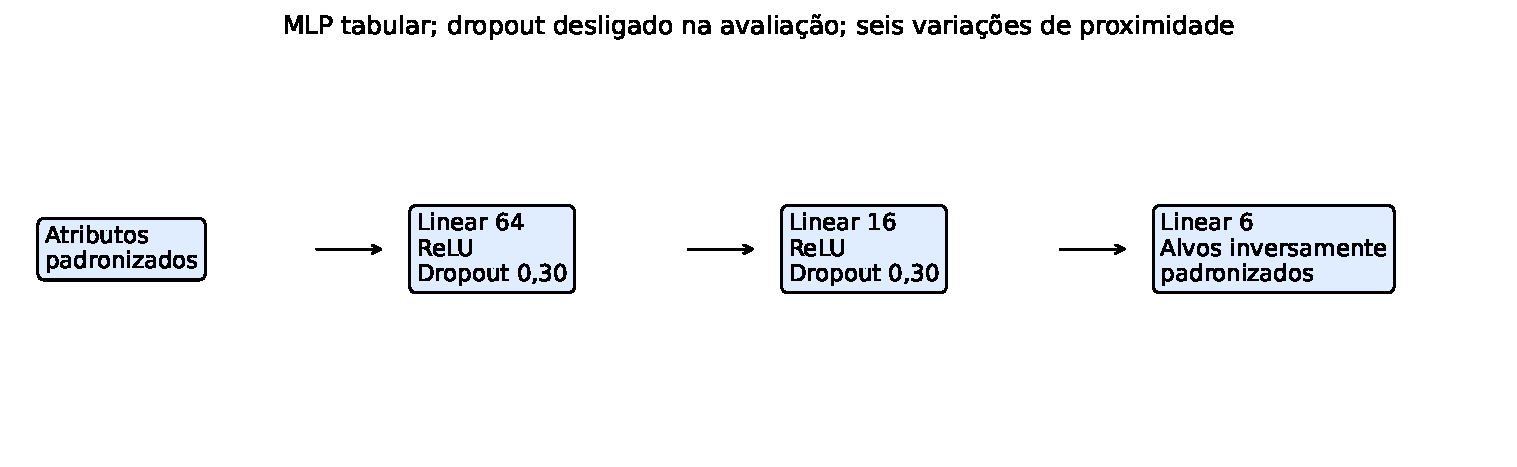
\includegraphics[width=.95\linewidth]{figuras/metodologia_mlp.pdf}
\caption{MLP tabular: duas camadas ocultas, dropout no treino e seis saídas de variação de proximidade. O número de atributos depende da representação angular documentada.}
\label{fig:mlp-revisada}
\end{figure}
As Figuras~\ref{fig:grupos-revisados} e~\ref{fig:mlp-revisada} distinguem os descritores observados da arquitetura que os recebe. Os comandos reativos são entradas do eixo tabular, não da rede monocular densa.

\section{Notebook de análise}

O notebook carrega os pares de diretórios, verifica a qualidade temporal e constrói as entradas e os alvos. Valores não finitos recebem zero após o carregamento. A curva de aprendizado usa conjuntos cumulativos de 9, 17, 25, 33 e 40 execuções, sempre preservando os casos anteriores e as mesmas duas execuções de validação e três de teste.

As entradas incluem duração e atraso de sincronização. Deltas de posição e atitude. Integrais e variações de giroscópio e acelerômetro. Comandos de risco, frenagem e desvio. Estatísticas do fluxo. Retenção de pontos. E descritores da diferença de imagem. O notebook também testa a representação dos ângulos por seno e cosseno.

O modelo principal é uma MLP multissaída em PyTorch. Entradas e alvos recebem padronização calculada somente no treino. A rede possui camadas ocultas de 64 e 16 unidades, ativação por unidade linear retificada (ReLU), \textit{dropout} de 0,30 após cada camada e saída linear com seis unidades. O treinamento usa Adam, taxa $10^{-3}$, regularização $L_2$ de $10^{-4}$, lotes de 64 amostras e erro quadrático médio (MSE) no espaço padronizado.

O limite é de 300 épocas. A parada antecipada monitora a MSE da validação, exige melhora superior a $10^{-4}$ e encerra após 50 épocas sem avanço. Ao final, os pesos da melhor época retornam ao modelo. O \textit{dropout} e a parada antecipada são técnicas usuais para reduzir sobreajuste \cite{Srivastava2014,Prechelt1998}.

A MLP, Random Forest, Extra Trees, cada marco da curva e cada configuração de ablação foram repetidos com as sementes 7, 21, 42, 84 e 123. As comparações entre MLP e árvores incluem IC95, teste $t$ pareado por semente e $d_z$ de Cohen \cite{Lakens2013}. O pareamento controla apenas a aleatoriedade computacional no mesmo conjunto fixo, sem equivaler a cinco novas coletas. Como existem cinco pares, seis alvos e nenhuma correção de multiplicidade, os testes são exploratórios.

A curva de crescimento, a tabela de modelos, os contrastes pareados e a ablação usam a mesma bateria final de cinco sementes da MLP completa com representação seno/cosseno. A curva de perda ilustra separadamente a MLP de referência com ângulos originais e semente 42.

\section{Núcleo da validação espacial}

A validação espacial foi separada do nó ROS~2 para permitir testes da geometria e do planejamento sem executar o simulador. O módulo recebe um mapa de profundidade, os parâmetros intrínsecos e uma transformação homogênea entre a câmera e o referencial local. A reprojeção segue o modelo de câmera pinhole e produz pontos no espaço tridimensional. A transformação câmera--corpo inclui o deslocamento da câmera no UAV. A pose do PX4 leva os pontos ao referencial NED.

Uma grade esparsa acumula evidências de espaço livre ao longo dos raios e de ocupação perto de seus extremos \cite{Elfes1989,Hornung2013}. A travessia conservadora dos segmentos inclui todos os voxels tocados, inclusive contatos em faces e arestas, para que diagonais não saltem obstáculos \cite{AmanatidesWoo1987}. Evidências ocupadas podem exigir repetição temporal, e sua remoção exige observações livres posteriores. A integração monocular ainda reserva uma margem antes do retorno e uma faixa de incerteza perto da profundidade prevista, reduzindo a chance de marcar como livre uma região que o modelo estimou longe demais.

Antes do planejamento, os voxels ocupados recebem uma expansão horizontal e vertical. O planejador A* trabalha somente no espaço observado como livre, com 6, 18 ou 26 vizinhos \cite{Hart1968}. O caminho discreto passa por simplificação de linha de visada e subdivisão em pontos de passagem. Cada segmento final volta a ser verificado na grade. Quando o destino global está fora da região observada, o sistema classifica voxels livres alcançáveis próximos da fronteira com o desconhecido, procura progresso em direção ao objetivo e mantém um afastamento configurado da fronteira \cite{Yamauchi1997}.

A execução possui verificações adicionais que não alteram o A*. Um novo plano não substitui um caminho ativo seguro sem oferecer progresso suficiente. A troca antecipada de ponto é vetada quando o segmento seguinte atravessa região desconhecida, ocupada ou inflada. Antes de uma recuperação, o veículo desacelera. Posições já percorridas formam uma memória de recuo. E janelas temporais limitam tentativas sem progresso. Cópias completas do estado da grade permitem repetir offline a decisão do planejador no estado em que ocorreu.

Essa separação mantém explícita a origem da profundidade. No modo \path{ground_truth_debug}, a profundidade do Gazebo valida geometria, mapa, planejamento e interface com o PX4. No modo \path{monocular_topic}, o mapa estimado recebe somente a saída do modelo monocular; a profundidade do Gazebo constrói um segundo mapa que atua como referência e veto experimental de segurança. Os dois mapas usam a mesma geometria e o mesmo planejador, mas podem ter margens de percepção diferentes.

\section{Estimador monocular e portões de validação}

O estimador parte do Depth Anything V2 ViT-S ajustado para profundidade métrica \cite{DepthAnythingV2}. Os pares RGB--profundidade gravados no cenário simulado \texttt{baylands} foram separados por execução completa. A v12 estabeleceu o ajuste inicial e as margens espaciais. A v13 reforçou penalizações para subestimações perigosas e superfícies falsas na altitude de voo. A v14 incorporou execuções completas da bateria final, e a v15 concentrou amostras difíceis de troncos e bordas de copas. A v16 ampliou o treino para 20 execuções completas; a v17 atacou superestimação localizada ligada a uma colisão análoga; e a v18 equilibrou esse risco com as subestimações que bloqueavam corredores livres. A v19 partiu da v18 e descongelou somente os dois últimos blocos do codificador, preservando os demais blocos. O refinamento usou duas épocas, lotes de duas imagens, AdamW com regularização de $10^{-2}$, taxa de $5\times10^{-7}$ na cabeça e $2\times10^{-8}$ no codificador, semente 42, 3.322 quadros efetivos de treino e 77 de validação. Treino e validação redimensionaram RGB e profundidade para $686\times518$ pixels, e a exportação ONNX manteve essa entrada.

A função objetivo combinou SILog, erro relativo absoluto ponderado por bordas e penalizações direcionadas:
\[
\begin{aligned}
\mathcal{L}={}&L_{\mathrm{SILog}}+0{,}30L_{\mathrm{rel}}
+0{,}08L_{\mathrm{cauda},5}\\
&+0{,}55(L_{\mathrm{sup}}+L_{\mathrm{inf}})\\
&+0{,}50(L_{\mathrm{cauda,sup}}+L_{\mathrm{cauda,inf}})\\
&+0{,}55L_{\mathrm{borda,sup}}+0{,}50L_{\mathrm{borda,inf}}\\
&+0{,}10L_{\nabla}.
\end{aligned}
\]
São válidos os pixels cuja referência é finita e está entre 0,5 e 30~m. A previsão é truncada inferiormente em 0,05~m e a referência, em 0,5~m. Para $g=\log \hat d-\log d$, o primeiro termo é
\[
L_{\mathrm{SILog}}=\sqrt{\overline{g^2}-0{,}5\,(\overline{g})^2+10^{-8}}.
\]
$L_{\mathrm{rel}}$ é a média ponderada de $|\hat d-d|/\max(d,1)$, dividida pela soma dos pesos de borda. $L_{\mathrm{cauda},5}$ é a média dos 10\% maiores erros positivos ponderados onde a referência está até 5~m. Superestimação e subestimação são médias ponderadas, normalizadas pela soma dos pesos, em profundidades até 20~m; cada cauda retém e promedia os 5\% maiores valores ponderados. Os termos de borda usam a mesma normalização entre pixels com gradiente relativo de pelo menos 0,10. O peso é $1+3{,}5\min(\nabla_r/0{,}10,1)$, sendo $\nabla_r$ o maior gradiente relativo horizontal ou vertical da referência. O termo $L_{\nabla}$ é a média do erro absoluto entre gradientes logarítmicos horizontal e vertical.

As quatro execuções de foco, já incluídas nas 20 execuções de treino, foram acrescentadas uma segunda vez. Foram selecionados exatamente 253 quadros difíceis em raio de 7~m, com alvo de um quadro por execução e divisão da guinada em faixas de $30^\circ$. Cada quadro foi acrescentado duas vezes, totalizando 506 inserções adicionais. Cada amostra de treino tinha probabilidade 0,5 de espelhamento horizontal conjunto de RGB e profundidade. Brilho e contraste eram sorteados uniformemente em $[0{,}85;1{,}15]$ e gama em $[0{,}9;1{,}1]$. Esses aumentos não foram aplicados na validação.

A avaliação não escolhe o modelo apenas por MAE ou erro relativo. Depois da validação por pixel, os quadros são repetidos offline para reconstruir os mapas e executar o A*. O portão espacial verifica falsos espaços livres, disponibilidade de caminho e colisões contra o mapa de referência. Os limites foram definidos ao fim do desenvolvimento e congelados antes da bateria final. Os critérios de colisão, falso espaço livre e caminho executável expressam requisitos conservadores de segurança. Os demais consideram a rota e a frequência de processamento. O mínimo de 100 quadros impede que um trecho curto e favorável aprove o modelo sem testar persistência do mapa e replanejamentos sucessivos. A execução primária foi usada como validação durante o treinamento da v19 e não é um teste independente. Depois do congelamento do artefato e dos parâmetros, os quatro conjuntos secundários foram reprocessados offline. Nenhum aprovou o portão completo. Por isso, o voo SITL monocular não foi iniciado.

Na configuração espacial final, a grade usa voxels de 0,75~m, conectividade 26, limiares de log-odds de 0,6 para ocupado e $-0,6$ para livre, raio horizontal inflado de 1,25~m e inflação vertical de 0,10~m. O mapa é atualizado a cada dez quadros, o replanejamento nominal ocorre a cada 1,5~s e o caminho em execução é revalidado a cada 0,25~s. Um plano é inseguro quando qualquer voxel enumerado conservadoramente ao longo de um segmento é desconhecido, ocupado ou pertence ao volume inflado. Uma colisão no replay ocorre quando um caminho executável intercepta a ocupação de referência.

\section{Dois fluxos de execução}

O fluxo legado mantém a lógica reativa baseada em fluxo óptico e publica \textit{setpoints} de velocidade. Ele continua disponível para reproduzir as análises tabulares e para trabalhos futuros sobre controle. O fluxo espacial seleciona \texttt{navigation\_mode=spatial\_astar}, desativa a influência dos comandos reativos e transforma os caminhos do A* em \textit{setpoints} de posição. Nesse segundo fluxo, sem controle reativo não significa ausência de controle físico: o PX4 ainda estabiliza o veículo e acompanha os pontos recebidos.

Por segurança, \texttt{spatial\_execute\_path} permanece falso nos arquivos YAML. Com esse valor, o sistema constrói mapas e planos sem armar. O voo com profundidade de referência exige ativação explícita desse parâmetro. O modo monocular possui um portão adicional: mesmo com a ativação explícita, sua bateria só deve ocorrer depois da aprovação offline. O roteiro completo e os comandos ficam em \path{docs/execucao_pipeline_espacial.md}.

\section{Considerações finais}

A implementação mantém coleta, análise tabular, percepção monocular e navegação espacial em componentes separados. Essa organização permite repetir decisões offline e examinar componentes sem refazer o voo. Ela não isola automaticamente a causa de cada falha: profundidade, sincronização, amostragem, atualização da ocupação e parâmetros do planejador ainda podem interagir. No replay, os quadros e as poses seguem a trajetória gravada; um caminho alternativo não gera novas observações. A avaliação offline caracteriza mapas e planos nessa sequência, sem reproduzir todo o comportamento do sistema em voo. Os resultados são apresentados no próximo capítulo.


No eixo tabular, a profundidade sintética fornece os alvos, sem integrar as entradas da MLP. Ela permite calcular a variação dos percentis P10, P50 e P90 e da porcentagem de pixels abaixo de 2, 5 e 10~m. No eixo espacial, a profundidade do Gazebo também alimenta diretamente a bateria de referência de mapa e A*, além de avaliar a alternativa monocular. Essa distinção separa a validação da geometria da avaliação do estimador.

Neste trabalho, esse planejamento não substitui o controle de voo. Ele serve como teste posterior: se a representação construída a partir da percepção não distingue espaço livre e obstáculos, o planejador também não conseguirá produzir um caminho seguro. Para reduzir o risco de colisão, as células ocupadas recebem uma margem compatível com o tamanho do drone e com a incerteza da estimativa. O PX4 continua responsável pela estabilização e pelo acompanhamento dos pontos de passagem. O trabalho não compara leis de controle.


Os limites temporais de 0,5 s e 0,08 s são escolhas operacionais do coletor para rejeitar intervalos longos e associações temporalmente distantes. Não foi demonstrada calibração ótima desses valores. Os hiperparâmetros documentam a configuração executada, sem representar busca sistemática ou garantia de generalização. As amostras reforçadas da v19 foram selecionadas por proximidade horizontal a posições de interesse, em raio de 7 m, com remoção de duplicados e exclusão das execuções reservadas. Não foram ordenadas pelo erro individual da rede.


A discretização de 0,75 m, as margens físicas e os coeficientes de perda representam configurações operacionais congeladas dos ensaios, não valores universais. Taxas pequenas e descongelamento parcial caracterizam um refinamento limitado do estimador pré-treinado. Os registros não demonstram uma busca ótima dos pesos da perda, do lote ou da discretização. A sensibilidade isolada de todos esses valores não foi estabelecida. O estudo preserva essa limitação em vez de atribuir retrospectivamente uma calibração não realizada.
